% chktex-file 2% chktex-file 29
% chktex-file 13
\documentclass{report}
\usepackage{setspace}
\usepackage[a4paper, total={7in, 10in}]{geometry}
\usepackage[fleqn]{amsmath}
\usepackage{empheq}
\usepackage{amssymb}
\usepackage{amsthm}
\usepackage{gensymb}
\usepackage[fleqn]{cases}
\usepackage{multicol}
\usepackage{color}
\usepackage{stix}
\usepackage{chngcntr}
\usepackage{tikz}
\usepackage{enumitem}
\usepackage{pgfplots}
\usepackage{etoolbox}
\usepackage{tikz-3dplot}
\usepackage{tkz-euclide}
\usepackage{enumitem}

\def\nswe#1#2#3{#1\,$#2^\circ\,#3'$}
\graphicspath{ {./assets/} }
\usetikzlibrary{calc,matrix,arrows}
\usetikzlibrary{decorations.pathmorphing,patterns, calligraphy, perspective,backgrounds}

\counterwithout{equation}{chapter}
\setlength{\columnseprule}{1pt}
\setlength{\columnsep}{24pt}
\setcounter{chapter}{16}
\hfuzz=100pt

\newcommand{\pgfplotsdrawaxis}{\pgfplots@draw@axis}
\makeatother
\pgfplotsset{only axis on top/.style={axis on top=false, after end axis/.code={
                    \pgfplotsset{axis line style=opaque, ticklabel style=opaque, tick style={thick,opaque},
                        grid=none}\pgfplotsdrawaxis}}}

\newtheorem{theorem}{Theorem}

\begin{document}

\makeatletter
\newcommand{\newparallel}{\mathrel{\mathpalette\new@parallel\relax}}
\newcommand{\new@parallel}[2]{%
    \begingroup
    \sbox\z@{$#1T$}% get the height of an uppercase letter
    \resizebox{!}{\ht\z@}{\raisebox{\depth}{$\m@th#1/\mkern-5mu/$}}%
    \endgroup
}
\makeatother

\newcommand{\sol}[1]{

    \noindent \textbf{Sol.}
}
\newcommand{\prooff}[1]{

    \noindent \textbf{Proof.}
}
\newcommand\m[1]{\begin{pmatrix}#1\end{pmatrix}}
\newcommand\vm[1]{\begin{vmatrix}#1\end{vmatrix}}
\newenvironment{amatrix}[1]{%
    \left(\begin{array}{@{}*{#1}{c}|c@{}}
        }{%
    \end{array}\right)
}
\newenvironment{cequation}{
    \makeatletter
    \setbool{@fleqn}{false}
    \makeatother
    \begin{equation*}
        }{\end{equation*}}

\begin{titlepage}
    \raggedleft{}
    \rule{1pt}{\textheight}
    \hspace{0.02\textwidth}
    \parbox[b]{0.75\textwidth}{

    {\Huge\bfseries Solution Book of \\[0.5\baselineskip] Mathematic}\\[2\baselineskip]
    {\large\textit{Ssnior 2 Part I}}\\[4\baselineskip]
    {\Large\textsc{MELVIN CHIA}}

    \vspace{0.5\textheight}

    {\noindent Written on 9 October 2022}\\[\baselineskip]
    }

\end{titlepage}

\doublespacing{}
\tableofcontents
\singlespacing{}
\newpage

\begin{multicols}{2}
    \begin{enumerate}
        \item The diagram below shows a right prism, its base $BCGF$ is a trapezoid, $BC = BF
                  = 12cm$, $FG = 16cm$. The lateral face $EFGH$ is a square, and is
              perependicular to another lateral face $ABFE$. Find:
              \begin{enumerate}
                  \item The angle formed by plane $CDHG$ and plane $EFGH$.
                  \item The angle formed by plane $ABH$ and plane $ABFE$.
              \end{enumerate}
              \begin{center}
                  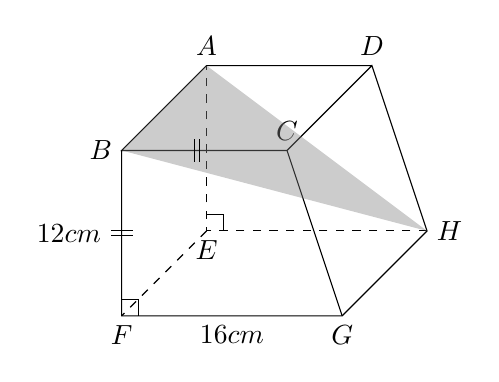
\begin{tikzpicture}[scale=1.4]
                      \draw (1.5,1.5,0) node [above] {$D$} --(0,1.5,0) node [above] {$A$} --(0,1.5,2) node [left] {$B$} --(1.5,1.5,2)node [above] {$C$} --(1.5,1.5,0) --(2,0,0) node [right] {$H$} --(2,0,2) node [below] {$G$} --(0,0,2) node [below] {$F$} node [midway, below] {$16cm$} --(0,1.5,2) node [midway, left=4pt] {$12cm$};
                      \draw (1.5,1.5,2)--(2,0,2);
                      \draw[dashed](2,0,0)--(0,0,0) node [below] {$E$}--(0,1.5,0);
                      \draw[dashed](0,0,0)--(0,0,2);
                      \fill [color=gray, opacity=0.4] (0, 1.5, 0) -- (0, 1.5, 2) -- (2, 0, 0) -- cycle;
                      \node (a) at (0,1.5,2) {};
                      \node (b) at (1.5,1.5,2) {};
                      \node (c) at (0,0,2) {};
                      \tkzMarkSegment[pos=.45,mark=||](a,b);
                      \tkzMarkSegment[pos=.5,mark=||](a,c);
                      \draw (0, 0.15, 0) -- (0.15, 0.15, 0) -- (0.15, 0, 0);
                      \draw (0, 0.15, 2) -- (0.15, 0.15, 2) -- (0.15, 0, 2);
                  \end{tikzpicture}
              \end{center}
        \item In the cuboid shown below, $BC = 8cm$, $CD = 6cm$, $BQ = 10cm$. Given that $M$
              is the midpoint of $PQ$. Find:
              \begin{enumerate}
                  \item The angle formed by line $MD$ and plane $PQBA$.
                  \item The angle formed by plane $AMD$ and plane $ABCD$.
              \end{enumerate}
              \begin{center}
                  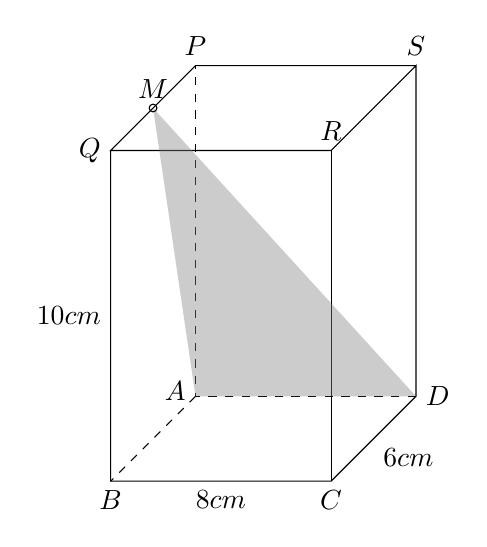
\begin{tikzpicture}[scale=1.4]
                      \draw (2,3,0) node [above] {$S$} --(0,3,0) node [above] {$P$} --(0,3,2) node [left] {$Q$} --(2,3,2)node [above] {$R$} --(2,3,0) --(2,0,0) node [right] {$D$} --(2,0,2) node [below] {$C$}  node [midway, below right] {$6cm$} --(0,0,2) node [below] {$B$}  node [midway, below] {$8cm$} --(0,3,2) node [midway, left] {$10cm$};
                      \draw (2,3,2)--(2,0,2);
                      \draw[dashed](2,0,0)--(0,0,0) node [above=2pt, left] {$A$}--(0,3,0);
                      \draw[dashed](0,0,0)--(0,0,2);
                      \fill [color=gray, opacity=0.4] (0, 3, 1) -- (0,0,0) -- (2, 0, 0) -- cycle;
                      \draw (0,3,1) circle (1pt) node [above] {$M$};
                  \end{tikzpicture}
              \end{center}
        \item The diagram below shows a pyramid with an isoceles triangle base. Given that
              $CD = CE = 5cm$, $ED = 6cm$, $ACD$ is a right-angled triangle, $B$ is a point
              on $AC$, $AD = 2cm$, $BC = 4cm$. Find:
              \begin{enumerate}
                  \item The angle formed by plane $BDE$ and plane $CDE$.
                  \item The angle formed by the plane $ADE$ and $CDE$.
              \end{enumerate}
              \begin{center}
                  \tdplotsetmaincoords{70}{70}
                  \begin{tikzpicture}[scale=0.6,tdplot_main_coords,declare function={d=6;}]
                      \path (0,0,0)       coordinate (A) node [left] {$E$}
                      (d,0,0)        coordinate (C) node [below] {$D$}
                      (d/2,{d*sqrt(3)/2},0)    coordinate (B) node [right] {$C$}
                      (d/2,{d*sqrt(3)/2 - 0.15} ,d-1.5) coordinate (F) node [right] {$B$}
                      (d/2,d/2 + 2,{d/sqrt(2) + 2}) coordinate (D) node [above] {$A$}
                      ($ (A)!0.5!(C) $) coordinate (M);
                      \foreach \p/\g in {A/-90,B/-90,C/-90,D/90}
                      \path (\p)+(\g:3mm);
                      \draw (F) circle (1.2pt);
                      \draw (D) -- (A) (D) -- (B) (D) -- (C) (A) -- (C) -- (B);
                      \draw [dashed] (A) -- (B);
                      \path (D) -- (F) node [midway, right] {$2cm$};
                      \path (B) -- (F) node [midway, right] {$4cm$};
                      \path (C) -- (B) node [midway, right=12pt, below=4pt] {$5cm$};
                      \path (A) -- (C) node [midway, left=14pt, below=-4pt] {$6cm$};
                      \fill [color=gray, opacity=0.4] (A) -- (C) -- (F) -- cycle;
                      \draw (d/2,{d*sqrt(3)/2},0.5) -- (d/2,{d*sqrt(3)/2 - 0.4} ,0.4) -- (d/2,{d*sqrt(3)/2 - 0.4} ,-0.1);
                      \tkzMarkSegment[pos=.45,mark=||](A,B);
                      \tkzMarkSegment[pos=.45,mark=||](B,C);
                  \end{tikzpicture}
              \end{center}
        \item The diagram below shows a regular pyramid with a square base. Given that $PQ =
                  15cm$, $PV = 20cm$. Find:
              \begin{enumerate}
                  \item The angle formed by linee $PV$ and plane $PQRS$.
                  \item The angle formed by the lateral faces and the base of the pyramid.
              \end{enumerate}
              \begin{center}
                  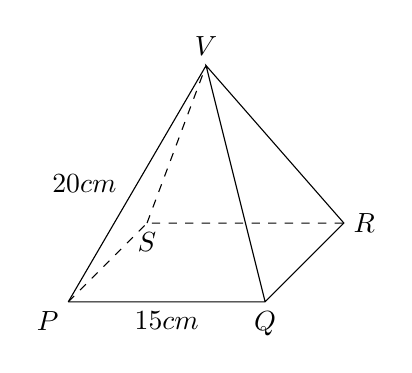
\begin{tikzpicture}
                      \tikzstyle{point}=[circle,thick,draw=black,fill=black,inner sep=0pt,minimum width=4pt,minimum height=4pt]
                      \node (a) at (0,0) {};
                      \node (b) at (2.5,0) {};
                      \node (c) at (3.5,1) {};
                      \node (d) at (1,1) {};
                      \node (e) at (1.75,3) {};
                      \draw (a.center) node [below left] {$P$} -- (b.center) node [below] {$Q$} node [midway, below] {$15cm$} -- (c.center) node [ right] {$R$} -- (e.center) node [above] {$V$} -- (b.center);
                      \draw (a.center) -- (e.center) node [midway, left=4pt] {$20cm$};
                      \draw[dashed] (a.center) -- (d.center) -- (c.center);
                      \draw[dashed] (d.center) node [below] {$S$} -- (e.center);
                  \end{tikzpicture}
              \end{center}
        \item The diagram below shows a right pyramid with lateral edges of $13cm$. Its base
              $ABCD$ is a rectangle with length of $12cm$ and width of $10cm$. Find:
              \begin{enumerate}
                  \item The angle formed by plane $VBC$ and plane $ABCD$.
                  \item The angle formed by plane $VCD$ and plane $ABCD$.
              \end{enumerate}
              \begin{center}
                  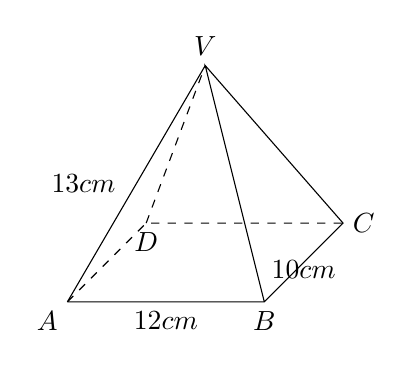
\begin{tikzpicture}
                      \tikzstyle{point}=[circle,thick,draw=black,fill=black,inner sep=0pt,minimum width=4pt,minimum height=4pt]
                      \node (a) at (0,0) {};
                      \node (b) at (2.5,0) {};
                      \node (c) at (3.5,1) {};
                      \node (d) at (1,1) {};
                      \node (e) at (1.75,3) {};
                      \draw (a.center) node [below left] {$A$} -- (b.center) node [below] {$B$} node [midway, below] {$12cm$} -- (c.center) node [ right] {$C$} node [midway, right=12pt, below=-4pt] {$10cm$} -- (e.center) node [above] {$V$} -- (b.center);
                      \draw (a.center) -- (e.center) node [midway, left=4pt] {$13cm$};
                      \draw[dashed] (a.center) -- (d.center) -- (c.center);
                      \draw[dashed] (d.center) node [below] {$D$} -- (e.center);
                  \end{tikzpicture}
              \end{center}
    \end{enumerate}
\end{multicols}
\end{document}